%%%%%%%%%%%%%%%%%%%%%%% CHAPTER - 1 %%%%%%%%%%%%%%%%%%%%\\
\chapter{Introduction}
\label{C1} %%%%%%%%%%%%%%%%%%%%%%%%%%%%
\graphicspath{{Figures/PDF/}{Figures/PNG/}}
\noindent\rule{\linewidth}{2pt}

%%%%%%%%%%%%%%%%%%%%%%%%%%%%%%%%%%%%%%%%%%%%%%%%%%%%%%%%%%%%%%%%%%%%%%%%%%%%%%%%%%%%%%%%%%%%%%%%%%%%%%%%%%%%%%%%%%%%%%%%%%%%%%%%%%%%%%
% \section{General Introduction} \label{S1.1} 
\noindent Wireless sensor network (WSN) are collection of number of sensor nodes having the property of auto-configuration and self-organization. Network architecture follows decentralization and is distributed in nature. WSN has a number of application in the areas of environmental monitoring like air, water and soil, structural monitoring, human activity, and behavioral monitoring, military surveillance, asset tracking and many more \cite{akyildiz2002wireless}. The advantage of WSN nodes is their small size and these can be placed at some place where surveillance by a wired network or human is not possible. These small nodes are deployed in thousands in number to monitor temperature, pressure etc. These nodes are always prone to physical damage because these are deployed in the open environment which is not protected. Self-organizing and auto-configuration in nature, limited battery, computation power, and bandwidth, distributed and decentralization, multihop communication in wireless medium, are some characteristics which may lead to exposing this network to many security attacks in all OSI model layers. To detect an inside attack intrusion detection system is introduced which can deal with wide range attacks in WSN.
\par
Security attack in WSN is either active or passive. In passive attack attacker generally, hide and collects data by tapping communication link but does not modify it. Traffic analysis, malfunctioning of a node, eavesdropping comes under passive attack. The active attack affects the operation of the network. An active attack can lead to termination or degradation in networking services. Denial-of-service (DoS, DDos), network jamming, wormhole, blackhole, sinkhole attacks are grouped in active attacks \cite{padmavathi2009survey}. Solutions to these attacks (active or passive) in any network involves prevention, detection, and mitigation \cite{fuchsberger2005intrusion}. In prevention step, the technique provides defense mechanism against attack i.e. it prevents the attack. Detection step comes into action when an attacker has found a way to pass prevention technique. This involves to detect or identify the node which has been attacked and compromised (being aware of the presence of attack). Mitigation aims to remove the attack detected in the detection step by taking action against the compromised node.
\par
IDS functionality is defined by the detection method which are mainly of two types - Anomaly-based, misuse-based. Anomaly-based technique tries to finds the deviation from normal behavior. To flag operation as an anomaly, the regular observation of system must be there to accommodate system changes. Misuse-based technique tries to detect previously known attack with high detection rate by comparing the new attack signature with known signatures.

\section{Wireless Sensor Netowrk}
Sensor nodes of WSN have capabilities to self-organize and auto-configure to create a network which can serve the purpose. WSN has several features like self-organization and auto-configuration in nature, distributed and decentralization, multi-hop communication etc. The first wireless network of sensors was used and created by US military to detect submarines of Soviet in 1950. From that time till now WSNs are used in various military to civil applications. Each sensor node consists of 5 main components - Sensing hardware, Transceiver, Micro-controller/CPU, Memory unit, Battery which supplies power to every unit. WSN are application specific so, different types of WSNs are used for different domain of application \cite{articleTypesWSN} as shown in Table \ref{tab:my-table2}.
\begin{table}[htp]
\centering
\caption{Types of WSN.}
\label{tab:my-table2}
\resizebox{\textwidth}{!}{%
\begin{tabular}{|p{1.25in}|p{1.25in}|p{1.5in}|p{1.5in}|}
\hline
\textbf{WSN Type} & \textbf{Deployment} & \textbf{Cost} & \textbf{Challenge} \\ \hline
Terrestrial & Structured or unstructured & Cheap & Management of hundreds and thousands of nodes \\ \hline
Underground & Structured & Expensive in node deployment and maintenance & Difficult to recharge battery, high attenuation and signal loss \\ \hline
Underwater & Structured or unstructured & Expensive in node deployment and maintenance & Communication - long propagation delay, sensor failure, Energy conservation \\ \hline
Multimedia & Structured or Unstructured & Low cost sensor nodes & high energy, bandwidth required with significant computation power \\ \hline
Mobile & Can move on their own & Expensive & Localization of nodes \\ \hline
\end{tabular}%
}
\end{table}

\section{Attacks in WSN} \label{S2.2}
WSNs are vulnerable to many attacks because of wireless multihop communication medium, decentralization, deployment in unprotected environment. Any attempt that tries to affect confidentiality, integrity and availability (CIA - Model) is defined as attack. Confidentiality ensures that only intended receiver has received message sent by sender and there is no unauthorized monitoring of message. Integrity ensures that message is not modified or altered. Availability ensures that when data is requested it is made available by source without much delay. It must consume less time in response.
\begin{figure}[ht]
\center	
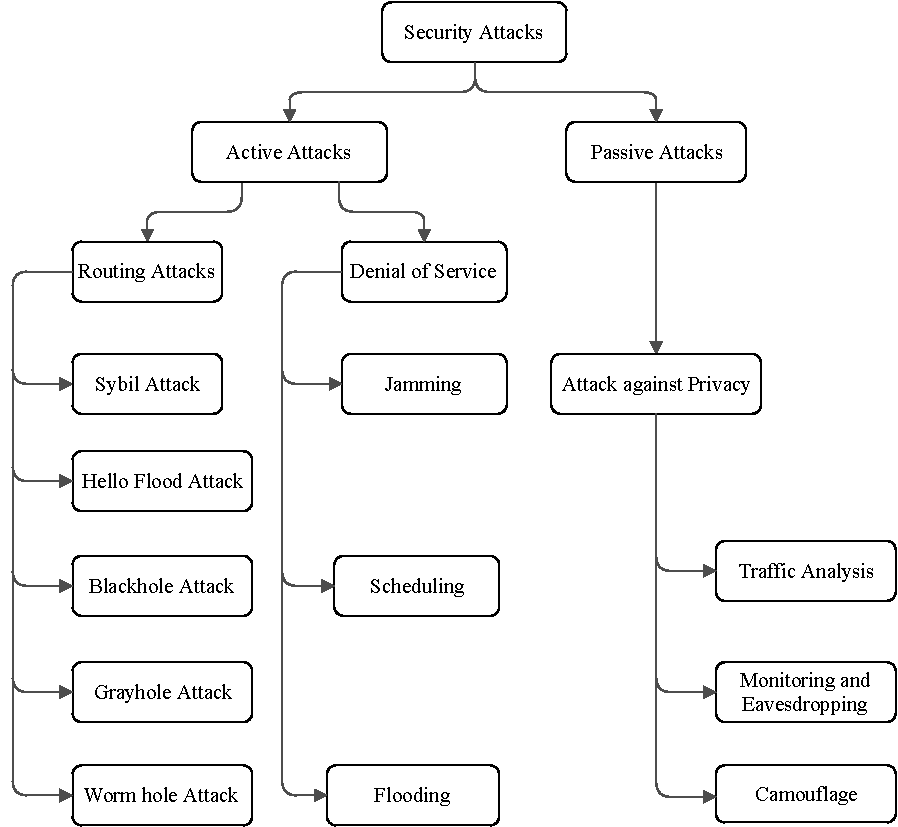
\includegraphics[width=5in, height=5in]{Figures/PDF/WSN-attacks.pdf}
\caption{Attacks in WSN.}
\label{WSN-Attacks}	
\end{figure}
\noindent
There are different threat model of attack in WSN \cite{roosta2006taxonomy}:
\begin{itemize}
  \item{ \textbf{Mote-class vs Laptop-class Attack} When the attack is on few sensor nodes inside WSN it is a mote-class attack and if the attack is done using a more powerful device, i.e. intense attack then it is a laptop-class attack.} 
  \item{ \textbf{Active Attack vs Passive Attack} An active attack is also known as a direct attack because it modifies the data being transferred between two nodes. Passive attack referred as less powerful, silent in nature than active attack. It is only used to collect information without modifying it. These attacks do not harm resources.}
  \item{ \textbf{Internal vs External Attack} These attacks are classified based on the domain of nodes as if the intruder node belongs to the network itself then it is an internal attack otherwise it is an external attack.}
\end{itemize}

\noindent

There are mainly 2 types of attacks \cite{wahid2015survey}- Active attack and Passive attack. Passive attacks are the attacks which are difficult to detect as compromised node in passive attack do not alter data. Passive attacks are only used for traffic monitoring or traffic analysis and do not harm the system. Passive attacks are big threat to confidentiality. Main emphasis in passive attack is to prevent attack rather than detection. Active attacks tries to modify and change the data transmitted on the network and always damages the system. Active attacks are threat to integrity and availability. Main emphasis in active attack is to detect attack. These attacks are found in the form of fabrication (e.g. Denial of Service -DoS attack), interruption (e.g. Masquerade attack), modification (e.g. replay attack).  Different type of attacks (active and passive attacks) in WSN are classified in Figure \ref{WSN-Attacks} \cite{nayak2015impact, abirami2013sybil, singh2014survey} -
\begin{enumerate}[label=\textbf{\roman*.}]
    \item \textbf{Wormhole Attack or Tunneling Attack} \cite{singh2014survey} Attacker tries to create a low latency link between two or more nodes which have better communication resources. These nodes can establish tunnels to communicate and data packets are tunnelled. This attack can change the network topology, can destruct packet, can change message stream by copying the packet at one place. After that, it rematches the same packet at different positions.
    
    \item \textbf{Sinkhole Attack }\cite{salehi2013detection} In sinkhole attack, the compromised node advertises fake routing to attract network traffic from neighboring nodes. Sinkhole attack is carried out by advertising fake high energy quality route to base station (BS). It is very likely that neighboring node to this compromised node will forward their data packets to this node which are destined to BS. Also, this attack can be used to trigger other attacks like selective forwarding attack. 

    \item \textbf{Blackhole Attack }\cite{wazid2013detection} Blackhole attack is carried out by reprogramming of some of network nodes such that these network do not forward data packets, according to routing algorithm, which are received. All data in this black hole region will be lost and it will cause delay and low throughput. This attack is hardly prevented because it shows original route information. This attack can be considered as denial-of-service attack.
    
    
    \item \textbf{Traffic Analysis }\cite{deng2005countermeasures} Traffic analysis is the process of examining data packet transfer from one sensor node to another node to extract information from the patterns. Attacker can find the location of BS by traffic analysis. Data in WSN routed from sensing nodes to BS via multihop communication follows same path until topology changes. By analyzing these traffic patterns location of BS can be found easily. Attacker once find the location, can directly attack BS.
    
    \item \textbf{Denial-of-Service (DoS or Distributed DoS) }\cite{patil2016attack} DoS attack is an attack in which the resource become so busy that it is unavailable to intended users. It stops a service from functioning efficiently, for e.g. internet site takes too long to respond in case of DoS attack. DoS attack aims  network’s bandwidth and connectivity so there is disruption in services of network. It directly affects the performance of the system. There are number of techniques available to prevent DoS attack which are mainly based on artificial intelligence, game theory, soft computing etc.
    \item \textbf{Replay Attack }\cite{sharma2017mitigating}
    It is a security failure in which firstly unauthorized information is stored and then it is re-transmitted to the receiver which can lead to duplicate transaction, false authentication, and many other unauthorized operations. Replay attack can be used as preliminary attack to many other DoS attack, by continuously observing and replaying the message exchange between two entities. Man-in-the-middle attack is a famous replay attack.

    \item \textbf{Jamming Attack }\cite{mpitziopoulos2009survey} Jamming attack targets the physical layer of the network and it can damage the whole network because the physical layer provides modulation, encryption, and many other important functions. Jamming in WSN carried out by interfering with the radio frequencies that are used by network for communication. It can be viewed as special type of DoS attack.
    
    \item \textbf{Sybil Attack }\cite{ssu2009detecting} Sybil attack is threat to integrity of network as compromised node in this attack tries to forge many fake identities to change network protocols. This lead to believe that a genuine node has many neighbor. It is an internal, passive attack. When a system is hijacked and it starts claiming for multiple identities then its a case of sybil attack. This attack is generally found in a distributed peer to peer network. 
    
    \item \textbf{Selective forwarding attack }\cite{bysani2011survey} It is a type of blackhole attack, as it is also related to the dropping of the data packet. It is carried out by internal nodes by drop data packets, selectively. If all packets are dropped by a node then it is a blackhole attack. This attack is difficult to detect as there is always some data packet loss in WSN due to unreliability.
    
    \item \textbf{Scheduling attack }\cite{almomani2015performance} It is a type of DoS attack Which mainly occurs in setup phase of LEACH protocol. At the time of time-slot allotment to member nodes by cluster head (CH), attacker node acting as CH will allocate same time slot to many member nodes to send the data which will cause data collision.
    
    \item \textbf{Flooding attack }\cite{almomani2015performance} Flooding attack is carried out in LEACH protocol when compromised node sends large number of CH advertisement message with high energy. This will waste a lot of time to decide CH. Also, energy of the sensor nodes will be wasted in receiving these many number of messages.
\end{enumerate}

\subsection{Attacks on Different Layers of OSI Model}
WSN network architecture mainly follows OSI model. This section presents possible attacks on each layer \cite{lupu2009main}. Physical layer and Data-link layers are mainly compromised by using passive attacks. Physical layer is attacked by jamming, interceptions and eavesdropping attacks where data link layer is attacked by traffic analysis, traffic monitoring. Black hole, Sink hole and Wormhole attacks are used to attack network layer to affect resources and network performance actively. Flooding and network consumption are also attacks found in network layer. Transport layer finds difficulties in data corruption and repudiation where transport layer is attacked by session hijacking. There are some attacks in WSN which can affect more than one layer of OSI architecture. Dos, Replay are multilayer attacks.

\section{Limitations and Challenges of WSN} \label{WSNChallenges}
Sensor nodes in WSN collects data using their sensing hardware, compute or process this data using CPU, communicate with other nodes. This data is being further processed at CH and then forwarded to BS. WSN provides efficient and low cost solutions to bridge the gap between real world and electronic world. However, WSN should be able to manage and configure itself as there is no human intervention after node deployment. WSN nodes have limitation in their storage capacity, processing power, battery power due to which these network have certain limitations and faces several issues \cite{sharma2013issues}.
\begin{enumerate}[label=\textbf{\roman*.}]
    \item \textbf{Security }
    WSN nodes can be deployed where surveillance using wired network or human is not possible. Also, these nodes are deployed in hostile unprotected environment where security of data is a big concern. Security is a broad term can be classified to confidentiality, integrity and availability of data. To make sure authenticity of network various cryptographic and secure mechanism have been introduced that can provide security up to some extent for outsider attacks. Data should not be altered or changed as it plays important role to maintain integrity. If there is a compromised node inside the network then it should be detected and all other nodes must have information about this compromised node. To do this, one needs to install IDS.
    \item \textbf{Energy }
    Sensor nodes consumes energy in every operation like sensing, processing data, communication, etc. Power source of a sensor node is a battery which is very tough to be recharged or replaced due to geographic conditions and critical application environment. So, efficient use of power source is essential in order to ensure that sensor node is alive for further operations. Mainly, energy is consumed in sensing transducer, analog to digital converter, computing unit, transmission and receiver energy. To conserve energy some of the sensing nodes need to be idle/sleep mode. Clustering of sensors can also be applied in order to conserve energy.
    \item \textbf{Routing Protocol }
    Routing protocols in WSN are different from routing protocols of MANET because WSNs are data-centric, unique identification number can not be assigned to sensor nodes as assigned in MANET because sensor nodes are very large in number, requirement of sensor network is application specific. To conserve energy aggregation of data is desired. Design of routing protocol must support ad-hoc node deployment to form connection between two randomly deployed nodes. Protocol must use limited energy and computation power without losing accuracy.
    \item \textbf{Data Collection and Transmission }
    Sensor nodes performs data gathering task which includes periodic data collection by sensing environment, process data and then transmit it to BS or sink node. In data gathering process redundant data must not be processed more than once because it will consume energy. To save energy clustering routing algorithms can be applied so low energy nodes will transmit data to high energy nodes where all processing of data will take place before sending to base station.
    \item \textbf{Quality of Service (QoS) }
    QoS is a measure of the level of service provided by network. WSN are used in real-time and critical application so desired quality service is very important. Change in network topology makes it difficult to achieve desired level of QoS. These mechanisms to provide QoS, must be aware of the fact that WSN data is aggregated and processed at various nodes and there is unbalanced traffic in the network. Scalability in WSN must not have any effect on QoS. Sometimes it is possible that network uses more energy to provide desired level of QoS.
    \item \textbf{Limited storage and processing power }
    Sensor nodes have limited amount of memory to store any code or data. Any security, QoS mechanism must have limited code that can be stored in node’s memory. WSN supports in-network processing with limited CPU power. Reduction in communication cost can be done by avoiding processing of redundant data.
\end{enumerate}
Furthermore, finding locations of each sensor node in the network is a key challenge known as Localization problem. Localization process is mainly divided into two steps- target/source localization node self-localization. WSN architecture needs secure and energy efficient routing algorithms with good QoS. Addition or removal of sensor nodes in network must not affect its performance that is scalability with QoS. MAC layer issues, operating system, network  architecture, node deployment, decentralized management, fault tolerance, robustness, heterogeneity, real time operation, data aggregation and data dissemination are some issues that are to be considered while designing or deploying any WSN.

\section{Applications of WSN}
\begin{figure}[htbp]
\center	
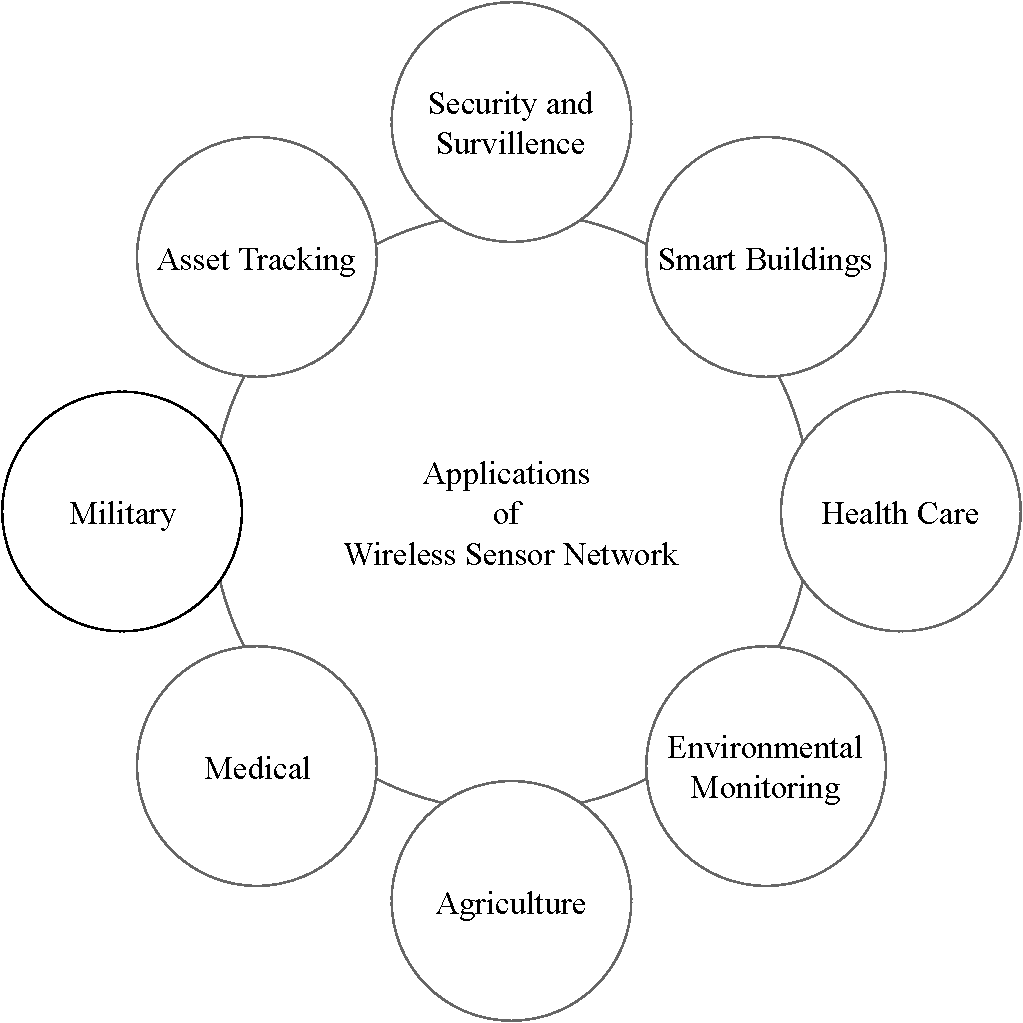
\includegraphics[width=4in, height=4in] {Figures/PDF/WSN-Applications.pdf}	
\caption{Applications of WSN.}
\label{WSN-Applications}	
\end{figure}
\newpage
WSNs are built using radio transceiver, sensing hardware, micro-controller, memory unit and battery. This sensor nodes senses data from surrounding and then this data is transmitted to main BS after processing. Features of WSNs like, mobility, fault tolerance, heterogeneity, auto-configuration, self-management, scalability etc are the reason of wide application range of WSN. Main application domains \cite{ramson2017applications} of WSN are shown in Figure \ref{WSN-Applications}. 
\par In agriculture, temperature and pressure with healthy environment is measured using WSN for better crop. Monitoring of environment helps to predict weather, monitoring of old buildings, bridges helps to avoid any accident. Asset tracking helps in finding the location of asset, vehicle tracking  helps in smart parking and to avoid congestion. In military, surveillance of enemy helps to plan perfectly.

\section{Motivation}
Application domain of WSN is very wide in the fields of medical to military and data plays very important role in every field. Intrusion is any activity in a network, which is not authorized and affects network's services, resources or data either passively or actively. Such activity if not prevented in the first line of defense in WSN security then IDS comes into play as the second line of defense. The network member nodes detects any suspicious behavior to detect intrusion. After detection, it cannot take action on it but it raises an alarm to the controller. IDS provides information to the controller about intruder information (identification of node or region, location, time and date of intrusion, an activity of intrusion, type of intrusion, etc). This information is used in the third line of defense i.e. in mitigating the attack.

\section{Problem Statement and Objectives}
In order to provide protection to WSNs many solutions such as cryptographic and secure routing, key exchange and authentication are proposed. These methods are used to provide security from outside attack up to some level but these cannot eliminate all security attacks. To detect an inside attack IDS is introduced which can deal with wide range of attacks in WSN. Main motive of this research is to design an IDS which can deal with intrusion attacks efficiently. Main focus in this research has been on high detection rate and low false positive rate.
\section{Organization of Dissertation}
The dissertation is structured in chapters. Chapters are organization as follows:
\\
\noindent Chapter \ref{C1} starts with brief introduction about WSN and IDS. Going forward, it gives a detailed overview of WSN followed by attacks in WSN. Various security attacks in wireless sensor network like DoS attack, replay attack, traffic analysis, blackhole, wormhole, sinkhole attacks etc has been discussed. Also, it is shown that which type of attack may occur on which layer of the OSI model. Different classes and types of attack are discussed in great detail. Then limitations and challenges faced by WSN are discussed. After that, brief introduction to applications of WSN is provided. This chapter ends with motivation for this research work, problem statement and objectives of this research. 
\par Chapter \ref{C4} provides a detailed description of IDS. This chapter starts with introduction of IDS and it's components. After that, classification  of IDS based on detection method, source of data etc. is discussed in great detail. Later in the chapter literature survey of various IDS is discussed. Various approaches of detection are discussed which are based on different fields like Neural network, support vector machine, cluster-based approaches etc. A tabular comparison of some detection techniques is also presented in this chapter which includes limitations and features of particular approach. Chapter ends with summary of limitations faced in current IDS.
\par Chapter \ref{C5} is focused on the proposed system for attack detection. It starts with the system model of proposed approach followed by dataset description used for training purpose. After that, proposed approach of neural network model is discussed. A systematic flow chart of algorithm is also discussed in this chapter. Steps of detection model are described in procedure section. This chapter ends with summary of proposed system.
\par Chapter \ref{C6} presents results of research work. It starts with discussing the simulation environment briefly followed by 3 comparison graphs of WSN energy model. After that, this chapter presents the 2 accuracy graphs of neural network model.
\par Chapter \ref{C7} concludes the dissertation. Conclusion explains the main findings and limitation of this research work with scope of future work.